\section{Introduction}	
    \label{sec:introduction}

% Detecting violent action from surveillance footage has plenty of merits. 
% Nowadays, almost every public place, i.e., school, bank, hospital, shopping mall, are under observation of security cameras. 
% As the number of security cameras is growing, the need for monitoring footage is also increasing. 
% It is arduous and expensive to monitor and detect violence in real-time from video data manually. 
% Moreover, it may take some time to inform the authority responsible for taking action in case of an emergency, while an automated violence detection system can do so almost immediately.
There are several advantages to detecting violent activity from surveillance video.
In today's world, security cameras may be found in practically every public area such as an office, hospitals, educational institutes, and shopping malls, among other places. As the number of security cameras grows, so does the demand for more sophisticated methods of monitoring the footages. Using manual methods to monitor and identify violence in real-time from video footage is time-consuming and costly. A further disadvantage is that it may take some time to notify the appropriate authorities responsible for taking action in the event of an emergency, while an automated violence detection system may do so nearly instantaneously.


When it comes to violence detection, it may be regarded as a subset of human action recognition, which seeks to recognize conventional human activity \cite{cheng2019rwf}.
% Violence detection can be considered a subset of human action recognition, which intends to identify standard human action~\cite{cheng2019rwf}. 
In image recognition, $I(h,w)$, the spatial characteristics $h$ and $w$ that offer information about the scene are generally extracted. In contrast, there is another dimension in video data $I(t,h,w)$ that contains information about the passage of time, which reveals the changes in spatial features with time.
It is required to extract both spatial and temporal information to detect violence from video data. 

\begin{figure}[t]
    \centering
    \subfigure[Movies fight detection dataset samples.]
    {
        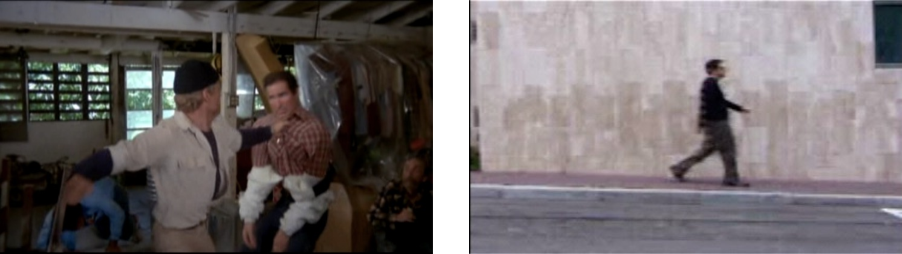
\includegraphics[width=0.4\textwidth]{new_images/sample-3.pdf}
        \label{fig:third_sub}
    }
    
    \subfigure[Hockey fight detection dataset samples.]
    {
        
\includegraphics[width=0.4\textwidth]{new_images/sample-2.pdf}
        \label{fig:second_sub}
    }
    
    \subfigure[RWF-2000 violence detection dataset samples.]
    {
        
\includegraphics[width=0.4\textwidth]{new_images/sample-1.pdf}
        \label{fig:first_sub}
    }
    \caption{Samples from different violent detection dataset.}
    \label{fig:sample_dataset}
\end{figure}

Previously, researchers employed a variety of feature extraction approaches, such as ViF~\cite{hassner2012violent_6}, STIPs~\cite{de2010violence_7}, iDT~\cite{wang2013action_9}, and fed the results to classic classification models, such as support vector machine (SVM).
Real-world settings, on the other hand, are complicated, as seen in Fig.~\ref{fig:sample_dataset}, and it is difficult to extract relevant information from hand-crafted feature descriptors.
Convolutional neural network (CNN), gated  recurrent  unit (GRU),  and  long  short-term  memory  (LSTM)  network  are deep learning-based approaches that have recently been demonstrated to be effective in learning interpretable and robust features from images, identifying spatial information, and achieving cutting edge results on image classification, segmentation, and other computer vision tasks~\cite{tan2019efficientnet,lin2017fpn}. 
Research has been carried out to extend the success of deep learning approaches to video analysis, with results that are at the state-of-the-art the field~\cite{eco14zolfaghari2018, 3dres101_hara2018can}.

The significance of extracted spatial and temporal features determines the success in violence detection as well as general human action recognition.
Modern approaches, in addition to RGB frames, depend on optical flow for temporal information. 
% However, in a real-time application, calculating optical flow becomes a bottleneck, making the model inappropriate for use in such circumstances~\cite{i3dcarreira2017quo}.
Furthermore, because of the high cost of computational complexity and the vast number of parameters, they are inefficient for any real-world application.
We believe that the problem lies in the way spatial and temporal characteristics are extracted in a current deep-learning model.
When developing the models, generally spatial and temporal characteristics are retrieved in a sequential manner, with temporal features extraction occurring after spatial data extraction. This results in a loss of information due to the fact that the features are not extracted from the same spatio-temporal position throughout the procedure.

% Success in violence detection, in general, human action recognition, lies in how significant extracted spatial and temporal features are.
% In most cases, modern methods rely on optical flow for temporal information along with RGB frames. 
% However, in a real-time application, computing optical flow becomes the bottleneck and makes the model unsuitable for applying in such situations~\cite{i3dcarreira2017quo}. 
% Moreover, the expensive computational complexity and large number of  parameters make then inefficient for any real-life deployment.
% According to our hypothesis, the issue exists in how spatial and temporal features are extracted in a modern deep learning model. 
% In the models, spatial and temporal features are extracted sequentially where, temporal features extraction follows spatial features. Thus, the features are not extracting from the same spatio-temporal point and a loss of information exists in the process.

% 	% 	%		%		%		% 	% 	%		%		%		%

%  Pipeline image   %

% 	% 	%		%		%		% 	% 	%		%		%		%	
	
	\begin{figure*}[!htb]
	\centering
	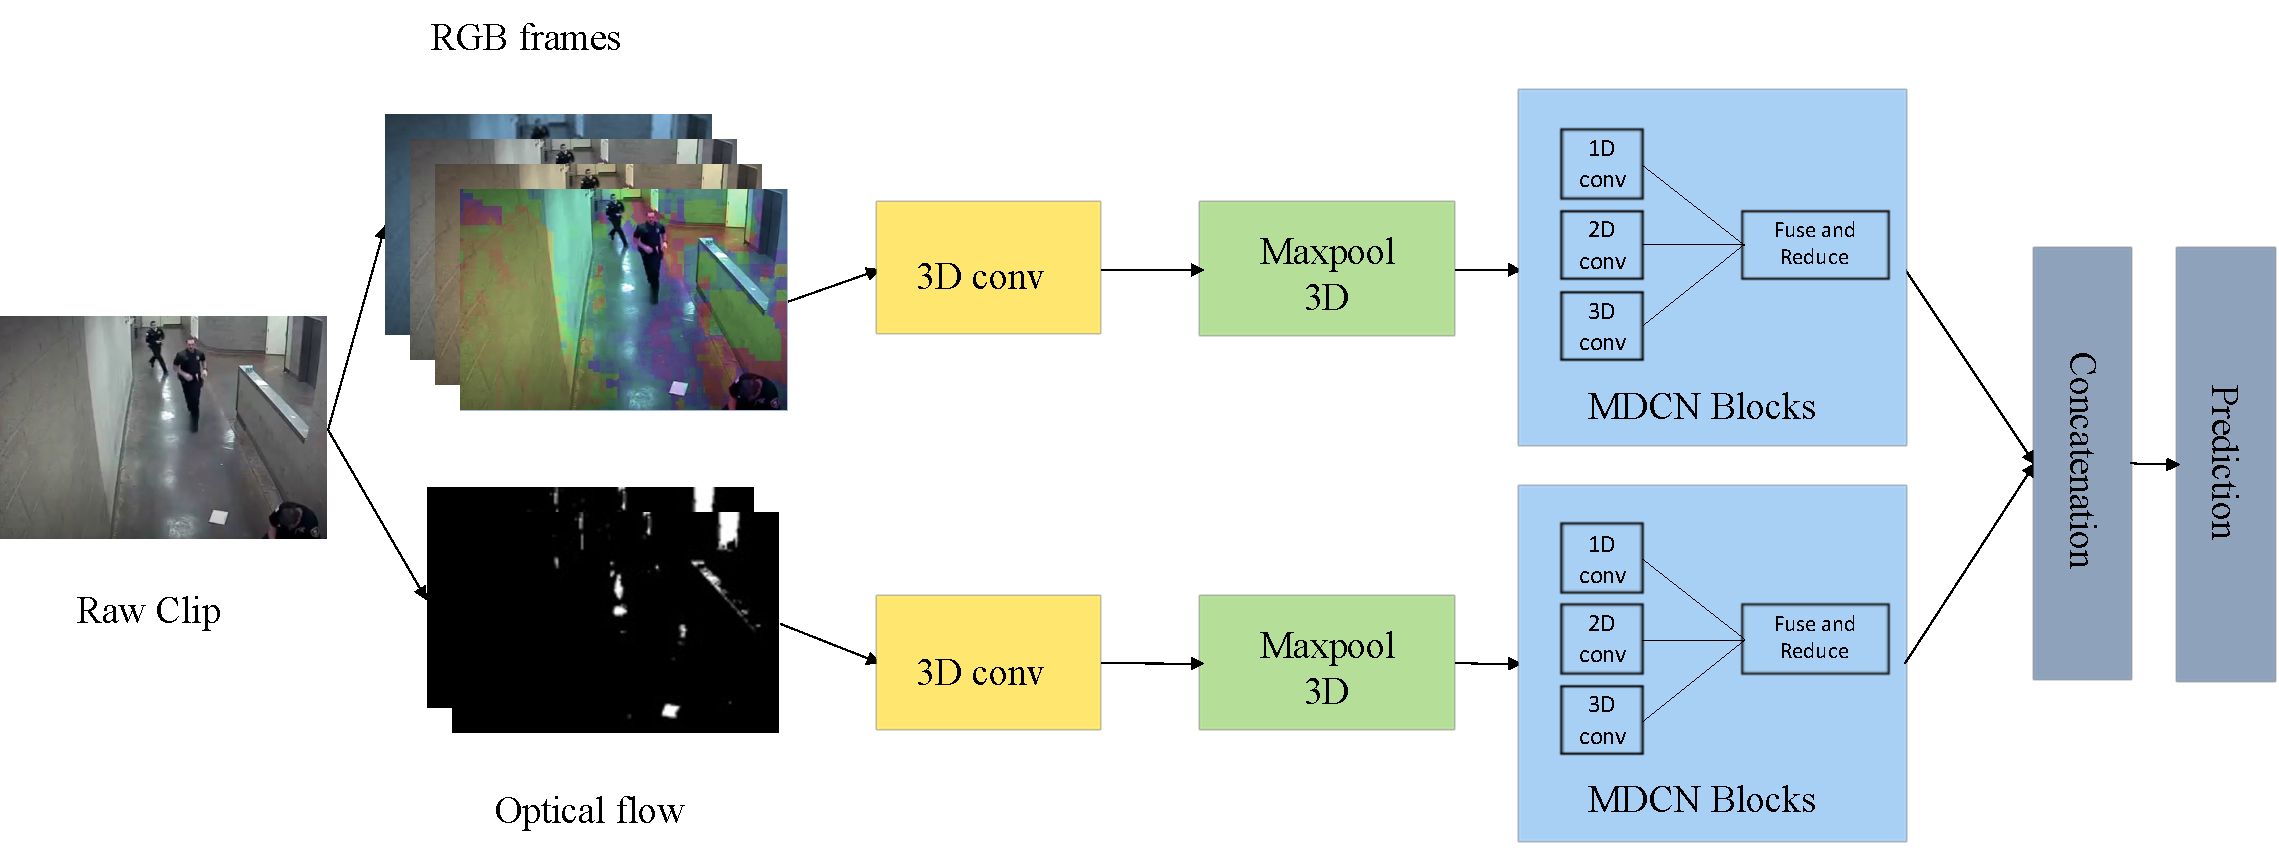
\includegraphics[width=0.9\linewidth]{new_images/pipeline.pdf}
	\caption{Overall pipeline of 2s-MDCN.}
	\label{fig:pipeline}
	\end{figure*}    

%subject to change
To address this problem, we propose a novel architecture for violence detection named the two-stream multi-dimensional convolutional network (2s-MDCN), as illustrated in Fig. ~\ref{fig:pipeline}.
Our proposed 2s-MDCN uses both RGB and optical flow as input and thus, the model has two separate branches for RGB stream and optical flow stream.
Our proposed model employs a fusion of multi-dimensional convolution processes to filter out spatial and temporal data separately retrieved from the same spatio-temporal point, therefore minimizing information loss.
% Additionally, the reduced computational cost and small parameter size make it deployable.
Our proposed method employs optical flow along with the RGB frames.
To demonstrate the effectiveness of our model, we conduct extensive experiments on three benchmark datasets for violence detection, including RWF-2000 violence ~\cite{cheng2019rwf}, Hockey-fight~\cite{hockey_nievas2011violence} and Movies-fight~\cite{movie_nievas2011violence} dataset.
We also performed experiments with a single RGB stream and optical flow stream. Our experiments show that adding optical flow increased the model accuracy by a significant amount.
Despite having low parameters and less complexity, our model obtained state-of-the-art accuracy in violence detection benchmark datasets.

The primary contributions of this work can be summarized as follows:
\begin{itemize}
    \item We explored how important it is to coordinate temporal and spatial features in violence detection.
    \item We proposed 2s-MDCN, a novel architecture for violence detection which takes RGB frames and optical flow as input. Our model extracts temporal and spatial features independently of each other whereas, current models do that in a sequential fashion which may not be suitable to fully exploit the features.
    \item Finally, this work can be considered a strong baseline for violence detection as our model achieved state-of-the-art accuracy in the largest violence detection dataset. We hope our baseline is helpful for future work in violent action detection.
\end{itemize}